\chapter{Технологическая часть}

\section{Средства реализации}

Для программной реализации шифровальной машины был выбран язык Python. В данном языке есть все требующиеся инструменты для данной лабораторной работы.

\section{Реализация алгоритма}

В листингах~\ref{lst:keygen}~---~\ref{lst:edcrypt} представлена реализация алгоритма RSA.

\begin{center}
\captionsetup{justification=raggedright,singlelinecheck=off}
\begin{lstlisting}[label=lst:keygen,caption=Генерация ключей]
def is_prime(n: int, k: int = 5) -> bool:
    if n <= 1:
        return False
    if n <= 3:
        return True
    if n % 2 == 0:
        return False
        
    d = n - 1
    r = 0
    while d % 2 == 0:
        d //= 2
        r += 1
        
    for _ in range(k):
        a = random.randint(2, n - 2)
        x = pow(a, d, n)
        if x == 1 or x == n - 1:
            continue
        for _ in range(r - 1):
            x = pow(x, 2, n)
            if x == n - 1:
                break
        else:
            return False
    return True

def generate_prime(bits: int) -> int:
    while True:
        num = random.getrandbits(bits)
        num |= (1 << bits - 1) | 1
        if is_prime(num):
            return num


def gcd(a: int, b: int):
    while b:
        a, b = b, a % b
    return a

def mod_inverse(a: int, m: int):
    def extended_gcd(a, b):
        if a == 0:
            return b, 0, 1
        gcd, x1, y1 = extended_gcd(b % a, a)
        x = y1 - (b // a) * x1
        y = x1
        return gcd, x, y
        
    gcd, x, _ = extended_gcd(a, m)
    if gcd != 1:
        raise ValueError("Обратный элемент не существует")
    return x % m

KEY_SIZE = 1024
def generate_keys() -> tuple[tuple[int, int], tuple[int, int]] | None:
    try:
        bits = KEY_SIZE
        p = generate_prime(bits // 2)
        q = generate_prime(bits // 2)
        
        n = p * q
        phi = (p - 1) * (q - 1)
        
        e = 65537
        while gcd(e, phi) != 1:
            e = random.randint(2, phi - 1)
        
        d = mod_inverse(e, phi)
        
        public_key = (e, n)
        private_key = (d, n)
        
        print("Ключи успешно сгенерированы")
        return (public_key, private_key)
    except Exception as ex:
        print(f"Ошибка при генерации ключей: {str(ex)}")
        return None
\end{lstlisting}
\end{center}

\begin{center}
\captionsetup{justification=raggedright,singlelinecheck=off}
\begin{lstlisting}[label=lst:edcrypt,caption=Шифрование/расшифровка алгоритмом RSA]
STD_PUB_KEY_FILE = ".rsa.pub"
STD_PRIV_KEY_FILE = ".rsa.priv"

def encrypt_file(finput: str, foutput: str, fpub_key: str = STD_PUB_KEY_FILE):
    try:
        e, n = load_key(fpub_key)
        block_size = n.bit_length() // 8 - 1
        
        with open(finput, 'rb') as f:
            data = f.read()
        
        encrypted_blocks = []
        for i in range(0, len(data), block_size):
            block = data[i:i+block_size]
            num = int.from_bytes(block, 'big')
            encrypted_num = pow(num, e, n)
            encrypted_block = encrypted_num.to_bytes((n.bit_length() + 7) // 8, 'big')
            encrypted_blocks.append(encrypted_block)
        
        with open(foutput, 'wb') as f:
            for block in encrypted_blocks:
                f.write(block)
        
        print("Файл успешно зашифрован!")
    except Exception as ex:
        print(f"Ошибка при шифровании: {str(ex)}")

def decrypt_file(finput: str, foutput: str, fpriv_key: str = STD_PRIV_KEY_FILE):
    try:
        d, n = load_key(fpriv_key)
        block_size = (n.bit_length() + 7) // 8
        
        with open(finput, 'rb') as f:
            data = f.read()
        
        decrypted_data = bytearray()
        for i in range(0, len(data), block_size):
            block = data[i : i + block_size]
            num = int.from_bytes(block, 'big')
            decrypted_num = pow(num, d, n)
            decrypted_block = decrypted_num.to_bytes((n.bit_length() // 8 - 1), 'big')
            decrypted_data.extend(decrypted_block)
        
        with open(foutput, 'wb') as f:
            f.write(decrypted_data)
        
        print("Файл успешно расшифрован!")
    except Exception as ex:
        print(f"Ошибка при шифровании: {str(ex)}")
\end{lstlisting}
\end{center}

\clearpage

\section{Пример работы программы}

На рисунке~\ref{fig:tex} представлен пример работы программы на текстовом фале.

\begin{figure}[h]
    \centering
    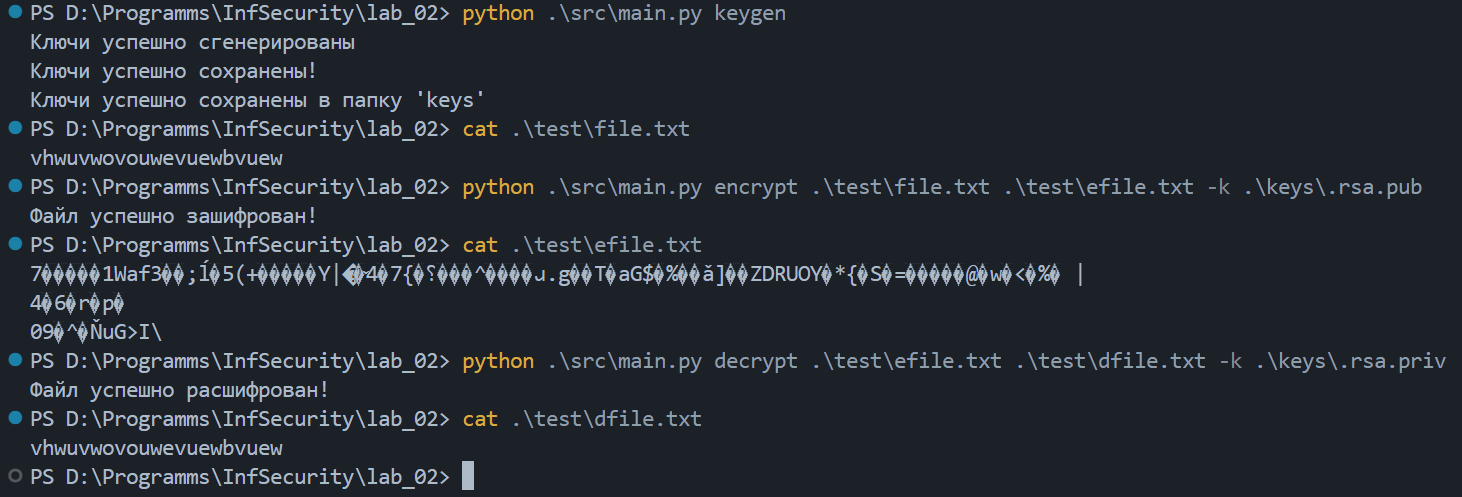
\includegraphics[width=1\linewidth]{images/tex.png}
    \caption{Пример работы программы на текстовом файле}
    \label{fig:tex}
\end{figure}

На рисунках~\ref{fig:zex}~---~\ref{fig:zd} представлен пример работы программы на zip-фале.

\begin{figure}[h]
    \centering
    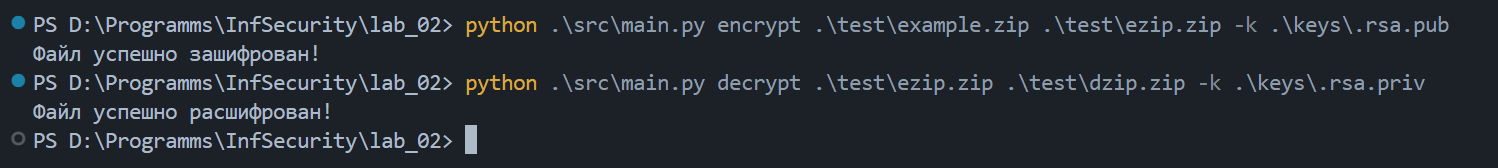
\includegraphics[width=0.9\linewidth]{images/zex.png}
    \caption{Шифрация/дешифрация zip-файла}
    \label{fig:zex}
\end{figure}

\begin{figure}[h]
    \centering
    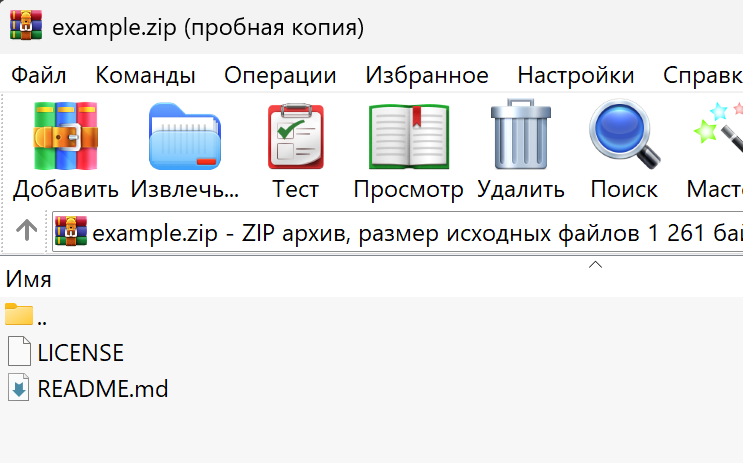
\includegraphics[width=0.6\linewidth]{images/fzip.png}
    \caption{Пример zip-файла}
    \label{fig:z1}
\end{figure}

\begin{figure}[h]
    \centering
    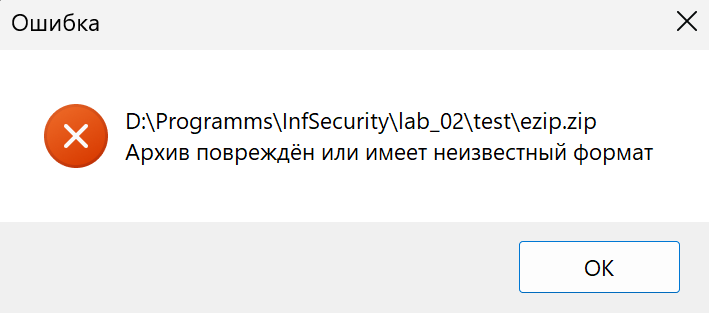
\includegraphics[width=0.6\linewidth]{images/ezip.png}
    \caption{Зашифрованный zip-файл}
    \label{fig:ze}
\end{figure}

\begin{figure}[h]
    \centering
    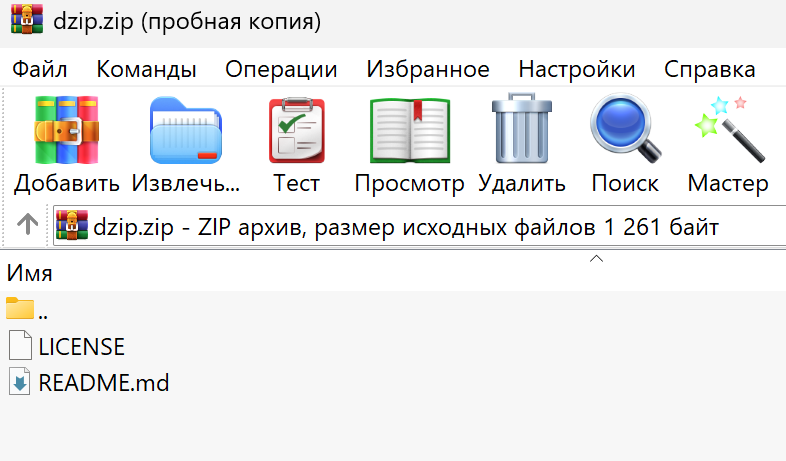
\includegraphics[width=0.6\linewidth]{images/dzip.png}
    \caption{Дешифрованный zip-файл}
    \label{fig:zd}
\end{figure}
